\documentclass[11pt]{article}

\usepackage[utf8]{inputenc}
\usepackage[T1]{fontenc}
\usepackage[margin=1in]{geometry}
\usepackage{amsmath}
\usepackage{amssymb}
\usepackage{graphicx}
\usepackage{booktabs}
\usepackage{xcolor}
\usepackage[colorlinks=true,linkcolor=black,urlcolor=blue]{hyperref}
\usepackage{parskip}

\graphicspath{{outputs/}}

\title{\vspace{-1.5em}CSc 8830 Computer Vision, Module 3\\[0.3em]
\large Image Blurring by Filtering: Spatial Domain vs Fourier Domain}
\author{Siri Bikkasani \\ Georgia State University}
\date{Fall 2026}

\begin{document}
\maketitle

\noindent GitHub repository: \url{https://github.com/siri423/Module3-ImageFiltering}

\section{Objective}

There are two parts to this assignment. First, implement image blurring using a
filtering approach, meaning I convolve the image with a small blur kernel and
write that convolution myself. Second, show that a spatial filter gives the same
result as its Fourier domain version, that is, that convolution in space is the
same as multiplication in frequency, and use my own implementation as the
evidence for it.

Everything runs as one Streamlit web app (\texttt{app.py}) where each part is
reachable from a tab, with the actual work done in a small set of commented
Python files under \texttt{src/}.

\section{Implementation: blurring by filtering}

Blurring an image means replacing every pixel with a weighted average of the
pixels around it. The weights are held in a small grid called a kernel. Sliding
that kernel across the image and taking the weighted sum at each spot is a 2D
convolution:
\begin{equation}
(f * g)(x,y) = \sum_{s}\sum_{t} f(s,t)\, g(x-s,\, y-t),
\end{equation}
where $f$ is the image and $g$ is the kernel. I built two kernels, both scaled so
their weights add up to $1$ (that keeps the brightness of the picture the same):

\begin{itemize}
\item A box kernel, where every weight is equal, so it is a plain average of the
neighbours.
\item A Gaussian kernel, where the weights follow a bell curve, so the centre
pixel counts most and the effect fades towards the edges. This gives a smoother,
more natural looking blur:
\begin{equation}
G(x,y) = \frac{1}{2\pi\sigma^2}\, e^{-(x^2 + y^2)/(2\sigma^2)}.
\end{equation}
\end{itemize}

\begin{figure}[h]
\centering
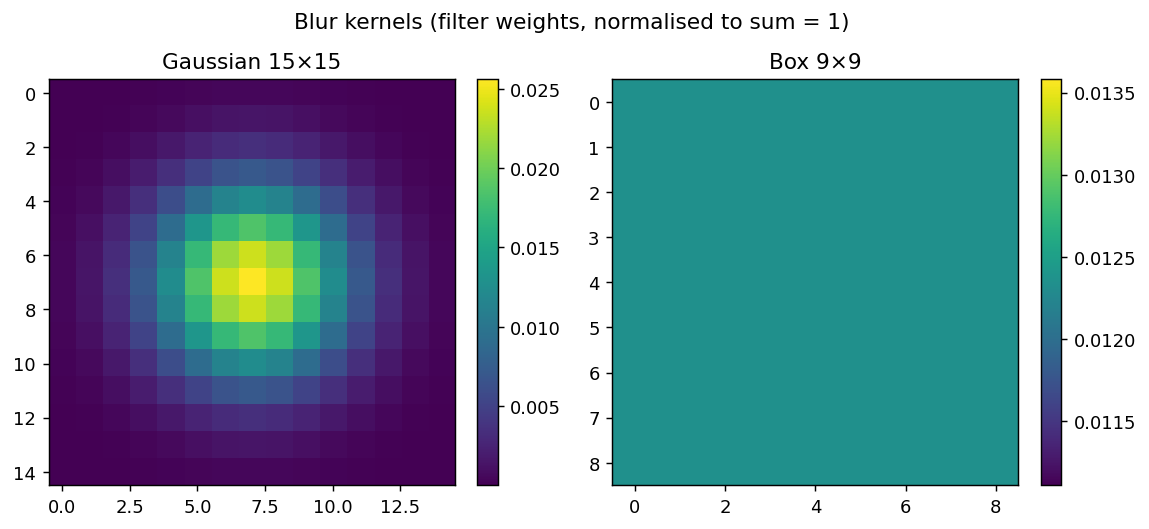
\includegraphics[width=0.72\textwidth]{fig_kernels.png}
\caption{The two blur kernels (the filter weights). The Gaussian keeps most of
its weight in the centre, and the box spreads it out evenly.}
\end{figure}

\subsection{The spatial convolution}

The convolution is in \texttt{src/spatial.py} and does not use any library blur
function. There is a plain nested loop version that states the definition
directly, and a faster version that gives the same answer by looping over the few
kernel positions instead of over every pixel:
\begin{verbatim}
for i in range(kh):
    for j in range(kw):
        # padded[i:i+H, j:j+W] is the image shifted by (i, j)
        out += kflip[i, j] * padded[i:i+H, j:j+W]
\end{verbatim}
The kernel is flipped first so this is true convolution rather than correlation
(for a symmetric blur kernel the two are the same). Image borders are handled by
zero padding, which I use for the proof because it makes the operation a linear
convolution, or by mirroring the edge for a nicer looking plain blur.

\begin{figure}[h]
\centering
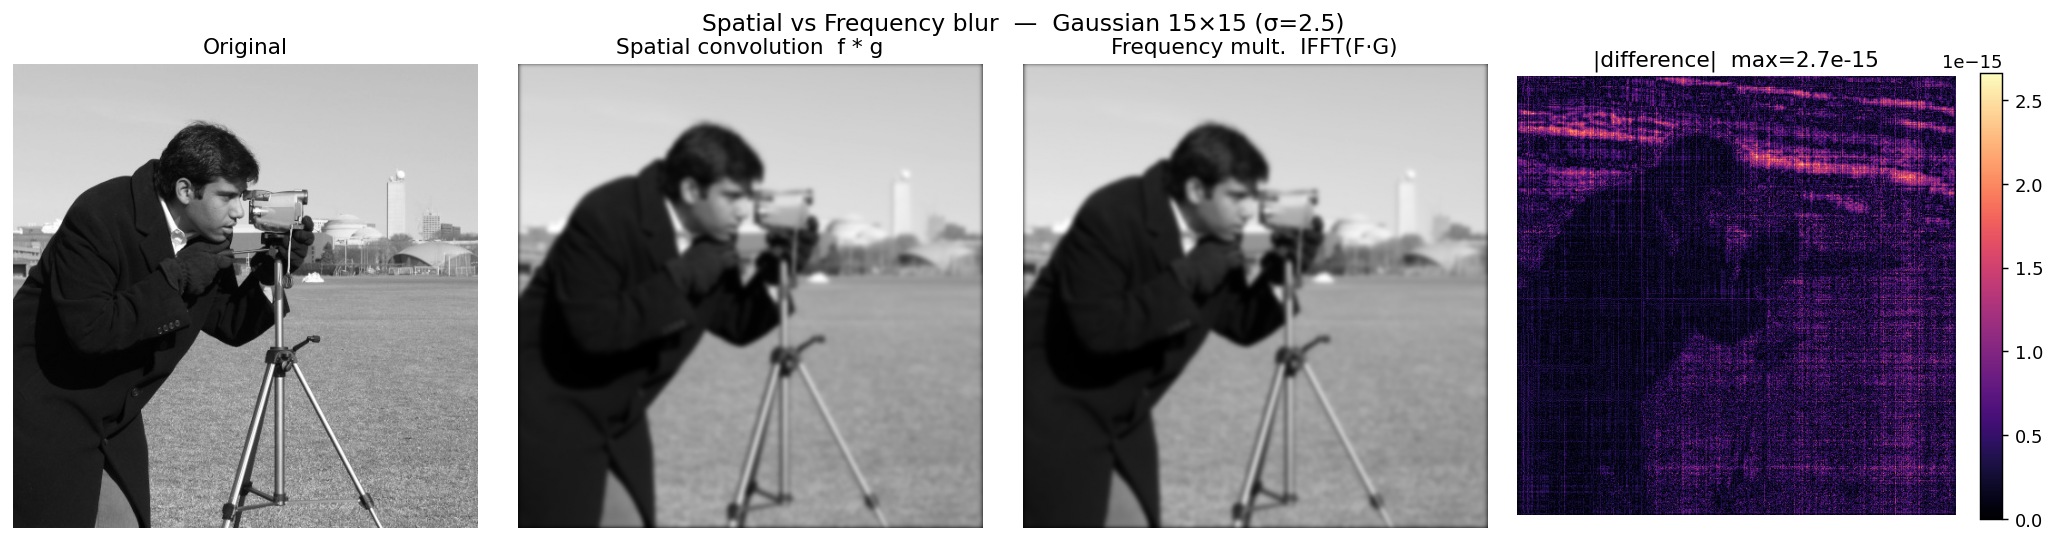
\includegraphics[width=\textwidth]{fig_comparison_gaussian.png}
\caption{The cameraman test image blurred with a Gaussian $15\times15$ kernel.
Panels 2 and 3 are the two methods from Section 3, and panel 4 is their
difference, discussed in Section 5.}
\end{figure}

\section{Theory: the Convolution Theorem}

The 2D Discrete Fourier Transform (DFT) of an $M\times N$ image is
\begin{equation}
F(u,v) = \sum_{x=0}^{M-1}\sum_{y=0}^{N-1} f(x,y)\,
e^{-j 2\pi (ux/M + vy/N)}.
\end{equation}
The Convolution Theorem says that convolution in one domain matches element-wise
multiplication in the other:
\begin{equation}
\boxed{\; f * g \;\;\Longleftrightarrow\;\; F \cdot G \;}
\end{equation}
So the blur can be done either by sliding the kernel (Section 2) or entirely in
the frequency domain:
\begin{equation}
f * g \;=\; \mathcal{F}^{-1}\!\left\{\, \mathcal{F}\{f\}\cdot \mathcal{F}\{g\}\,\right\}.
\end{equation}
This is what \texttt{src/frequency.py} does: take the FFT of the image, take the
FFT of the kernel, multiply the two spectra, and take the inverse FFT.

\subsection{Proof}

It is enough to prove the 1D case, since the 2D transform is just the 1D
transform applied along the rows and then the columns. Write $\omega = e^{-j2\pi/N}$
and let $y[n] = \sum_{m} f[m]\, g[(n-m)\bmod N]$ be the circular convolution. Its
DFT is
\begin{equation}
Y[k] = \sum_{n=0}^{N-1}\left(\sum_{m=0}^{N-1} f[m]\, g[(n-m)\bmod N]\right)\omega^{nk}.
\end{equation}
Substitute $p = (n-m)\bmod N$, so $n = m + p$, and because $\omega^{N} = 1$ we have
$\omega^{nk} = \omega^{mk}\omega^{pk}$. The double sum then splits into two:
\begin{equation}
Y[k] = \left(\sum_{m} f[m]\, \omega^{mk}\right)\left(\sum_{p} g[p]\, \omega^{pk}\right)
     = F[k]\, G[k].
\end{equation}
So the transform of a convolution is the product of the transforms. The other
direction, multiplication in space matching convolution in frequency, follows the
same way using the inverse transform.

\subsection{Linear vs circular convolution}

The plain FFT gives a circular convolution, where the kernel wraps around the
image edges. To reproduce the ordinary zero padded (linear) convolution from
Section 2, both arrays are zero padded to size $(M+k-1)\times(N+k-1)$ before
transforming (with $k$ the kernel width), and the middle is cropped out
afterwards. This is the reason the two methods match to rounding error in
Section 5 instead of only looking similar.

\subsection{Why a blur kernel blurs}

A box or Gaussian kernel is a low pass filter. Its transform $G(u,v)$ is large
near the origin (low frequencies) and small far away (high frequencies). Forming
$F\cdot G$ keeps the smooth, slowly changing content and cuts the fine detail and
sharp edges, which is what blurring means.

\begin{figure}[h]
\centering
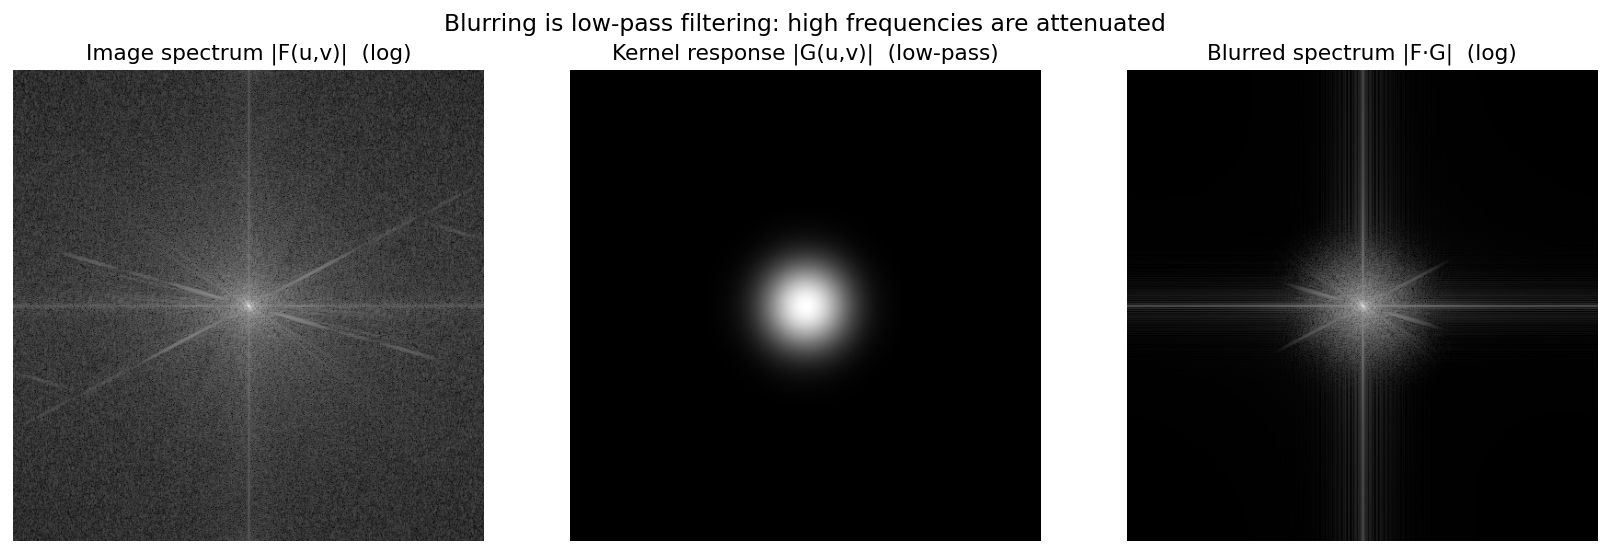
\includegraphics[width=\textwidth]{fig_spectra_gaussian.png}
\caption{The frequency domain view (log magnitude spectra). Left: the image
spectrum. Middle: the kernel response, bright in the centre, which is a low pass
filter. Right: the blurred spectrum, with the high frequencies clearly reduced.}
\end{figure}

\section{Worked example by hand}

To make the theorem concrete, here is a small case done fully by hand and then
checked with the code. Take the length 4 signal and 2 tap filter
\begin{equation}
f = [\,1,\, 2,\, 0,\, 3\,], \qquad g = [\,1,\, 1,\, 0,\, 0\,].
\end{equation}

\textbf{(a) Direct circular convolution.} Here $y[n] = f[n] + f[n-1]$ with the
indices taken mod 4:
\begin{equation}
y = [\,1{+}3,\; 2{+}1,\; 0{+}2,\; 3{+}0\,] = [\,4,\, 3,\, 2,\, 3\,].
\end{equation}

\textbf{(b) Through the DFT.} Using $\omega = e^{-j2\pi/4} = -j$, so the powers of
$\omega$ are $1, -j, -1, j$,
\begin{equation}
F = [\,6,\; 1{+}j,\; -4,\; 1{-}j\,], \qquad G = [\,2,\; 1{-}j,\; 0,\; 1{+}j\,].
\end{equation}
Multiplying element by element,
\begin{equation}
F\cdot G = [\,6\cdot 2,\; (1{+}j)(1{-}j),\; (-4)(0),\; (1{-}j)(1{+}j)\,]
        = [\,12,\, 2,\, 0,\, 2\,].
\end{equation}
The inverse DFT of $[\,12, 2, 0, 2\,]$ is
\begin{equation}
y = \tfrac{1}{4}\,\mathcal{F}^{-1}\{F\cdot G\} = [\,4,\, 3,\, 2,\, 3\,],
\end{equation}
which is the same as the direct convolution in part (a). Multiplying the two
transforms and inverting reproduces the convolution exactly.

As a quick 2D check, convolving the patch $[[10,20,30],[40,50,60],[70,80,90]]$
with a normalised $3\times3$ box kernel gives a centre value of
$\tfrac{1}{9}(10 + 20 + \dots + 90) = 50$, which is just the average of the
patch, as expected.

\section{Experimental validation}

\textbf{Method.} The cameraman image is blurred with the same kernel two ways: the
hand written spatial convolution from Section 2, and the Fourier domain
multiplication from Section 3. The two outputs are then compared pixel by pixel.
If the theorem holds they should be equal apart from floating point rounding.

Panels 2 and 3 of Figure 2 are the two results, and panel 4 is their absolute
difference, whose largest value is about $10^{-15}$, the scale of machine
rounding, so the images are the same. Repeating this across kernels and sizes
gives the table below.

\begin{table}[h]
\centering
\begin{tabular}{llrrr}
\toprule
Kernel & Size & max abs difference & MSE & PSNR (dB) \\
\midrule
gaussian & $3\times3$   & 2.00e-15 & 2.14e-31 & 306.7 \\
gaussian & $7\times7$   & 1.22e-15 & 7.11e-32 & 311.5 \\
gaussian & $15\times15$ & 2.66e-15 & 2.23e-31 & 306.5 \\
gaussian & $25\times25$ & 3.89e-15 & 4.02e-31 & 304.0 \\
box      & $3\times3$   & 1.78e-15 & 1.63e-31 & 307.9 \\
box      & $7\times7$   & 1.78e-15 & 1.03e-31 & 309.9 \\
box      & $15\times15$ & 6.99e-15 & 1.66e-30 & 297.8 \\
box      & $25\times25$ & 1.53e-14 & 8.31e-30 & 290.8 \\
\bottomrule
\end{tabular}
\caption{Difference between the spatial and Fourier results across settings.}
\end{table}

Across every setting the biggest pixel disagreement is between $10^{-15}$ and
$10^{-14}$, and the PSNR is around 290 to 312 dB. So spatial filtering and its
Fourier domain version give the same image, and convolution in space equals
multiplication in frequency. The small leftover is not an error in either method;
it is the buildup of 64 bit floating point rounding, and it grows slowly with the
kernel size (more terms in each sum), which is what you would expect.

\section{Repository and how to run}

\begin{verbatim}
Module3_ImageFiltering/
  app.py              Streamlit web app, all parts reachable here
  requirements.txt
  README.md
  src/
    kernels.py        box and Gaussian kernels
    spatial.py        hand written 2D convolution (the blur)
    frequency.py      FFT based filtering (multiply in frequency)
    compare.py        spatial vs frequency experiment and figures
    utils.py          load and save images
  data/sample.jpg     built in test image
  outputs/            result figures used in this report
\end{verbatim}

Run the web app (this is what the screen recording shows):
\begin{verbatim}
pip install -r requirements.txt
streamlit run app.py        then open http://localhost:8501
\end{verbatim}
Reproduce the experiment and figures from the command line:
\begin{verbatim}
python -m src.compare --kind gaussian --size 15
python -m src.compare --kind box --size 9
\end{verbatim}
Each requirement is shown in the app: blurring on the tab ``1. Blur an image'',
the spatial equals frequency proof on ``2. Spatial = Frequency'', and the theory
on ``3. Theory'' and in Sections 3 and 4 above.

\section{References}

\begin{itemize}
\item R. C. Gonzalez and R. E. Woods, \textit{Digital Image Processing}, 4th ed.
Chapter 3 on spatial filtering and Chapter 4 on filtering in the frequency
domain and the convolution theorem.
\item A. V. Oppenheim and R. W. Schafer, \textit{Discrete-Time Signal
Processing}, on the DFT and circular convolution.
\item NumPy FFT documentation, \texttt{numpy.fft}.
\end{itemize}

\end{document}
